\documentclass[lang=cn,11pt,a4paper,cite=authornum]{paper}

\title{编译原理与技术课程设计:Pascal-S编译器的设计与实现\\ 实验报告}
\author{李康童 \\ 2019211408 \and 班建龙 \\ 2019211368 \and 毛子恒 \\ 2019211397 \and 谢澳伦 \\ 2019211377 \and 李俊辉 \\ 2019211415 \and 乔永琦 \\ 2019211372}
\institute{北京邮电大学\ 计算机学院(国家示范性软件学院)}

\date{\zhtoday}

% 本文档命令
\usepackage{array}
\usepackage{threeparttable}
\newcommand{\ccr}[1]{\makecell{{\color{#1}\rule{1cm}{1cm}}}}
\nocite{*}

\begin{document}

\maketitle

\tableofcontents

\newpage

\section{需求分析}

我们设计并实现了\emph{s1mple-compiler},一个Pascal-S语言编译器。

\subsection{源语言说明}

Pascal-S是Pascal语言的真子集,它保留了Pascal语言的大部分功能。其文法描述见\ref{PascalS}节。

\subsection{目标语言说明}

LLVM是一种基于静态单一分配(Static Single Assignment,SSA)的中间表示(IR),它提供类型安全、低级操作、高灵活性以及清晰地表示所有高级语言的能力。 它是LLVM编译的所有阶段使用的通用代码表示。

LLVM IR以三种不同的形式出现:作为内存编译器的IR、作为磁盘上的二进制码表示以及作为人类可读的汇编语言表示。
LLVM IR为高效的编译器转换和分析提供强大的中间表示,同时实现自然的调试和可视化。三种不同形式的LLVM IR都是等价的。

LLVM IR的语法细节见\href{https://llvm.org/docs/LangRef.html}{LLVM Language Reference Manual}。

\subsection{功能描述}

\emph{s1mple-compiler}以Pascal-S语言源程序(.pas文件)作为输入,生成LLVM中间代码和可执行文件。

\subsection{实验环境}

\begin{itemize}
    \item Docker version 20.10.14
    \item Ubuntu 20.04.4 LTS
    \item ANTLR Parser Generator Version 4.9.3
    \item Ubuntu LLVM version 13.0.1
    \item Ubuntu clang version 13.0.1
    \item cmake version 3.16.3
\end{itemize}

\subsection{工具说明}

\paragraph{Docker} 为了实现组内快速的开发环境配置,我们构建了\href{https://www.docker.com/}{Docker}镜像,在Docker容器内进行项目的构建和运行。利用VSCode的\href{https://marketplace.visualstudio.com/items?itemName=ms-vscode-remote.remote-containers}{Remote - Container}插件和\href{https://marketplace.visualstudio.com/items?itemName=ms-vscode.cpptools-extension-pack}{C/C++ Extension Pack}插件,可以实现在VSCode内进入容器环境,以及代码高亮和自动补全等功能。

\paragraph{ANTLR} \href{https://www.antlr.org/}{ANTLR}是基于LL(*)算法实现的语法解析器生成器,使用自上而下(top-down)的递归下降LL剖析器方法。我们采用ANTLR实现了词法分析和语法分析,并生成了语法树。

\paragraph{LLVM} \href{https://llvm.org/}{LLVM}是一套编译器基础设施项目,包含一系列模块化的编译器组件和工具链。我们利用LLVM组件实现了中间代码生成、代码优化、可执行文件生成等功能。

\paragraph{其他工具} 使用\href{https://git-scm.com/}{Git}进行版本管理,使用\href{https://www.doxygen.nl/}{Doxygen}生成API文档,使用\href{https://cmake.org/}{CMake}构建项目。

\section{总体设计}

\subsection{技术路线}

前端部分采用ANTLR语法解析器,通过预定义的Pascal-S语法范式对输入的Pascal程序进行词法分析、语法分析,生成语法树;
然后借由ANTLR的Visitor模式遍历语法树,调用LLVM接口生成LLVM中间代码;
最后由clang优化中间代码、并且生成对应的可执行文件。

\subsection{实现方法}

我们的代码实现主要由以下三个部分构成:

\begin{enumerate}
    \item 通过ANTLR的语法规则定义Pascal-S的语法范式。
    \item 编写C++代码,通过Visitor模式访问语法树,利用LLVM IRBuilder构造LLVM IR。
    \item 利用shell脚本简单封装,实现自动化编译过程。
\end{enumerate}

\subsection{整体结构}

\emph{s1mple-compiler}的整体结构如\figref{fig:overview}。

\begin{figure}[htbp]
    \centering
    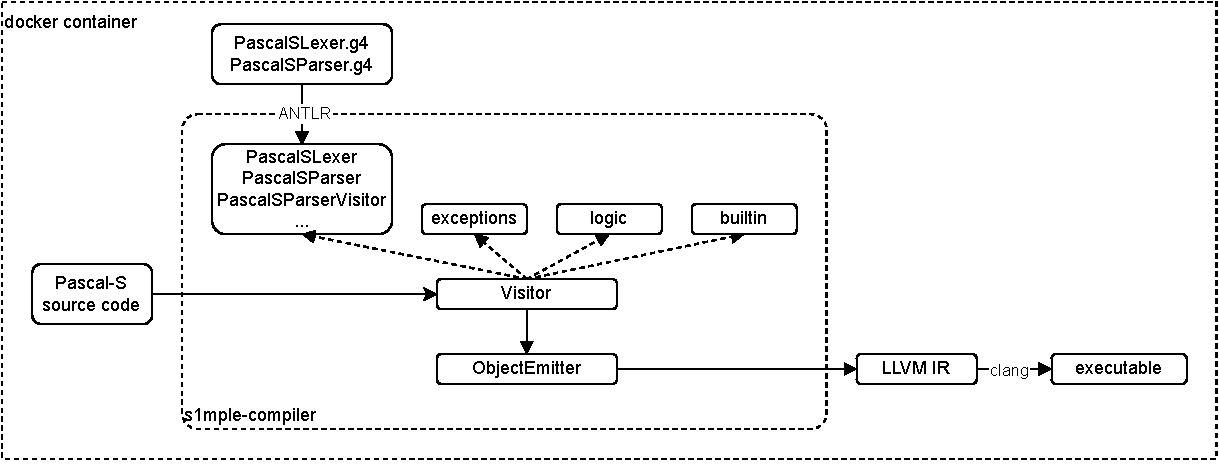
\includegraphics[width=\linewidth]{./Images/overview.pdf}
    \caption{整体结构\label{fig:overview}}
\end{figure}

\section{详细设计}

\subsection{词法、语法分析模块}

我们采用ANTLR的格式来描述\ref{PascalS}节的Pascal-S的词法和语法,分别见\href{run:../src/PascalSLexer.g4}{PascalSLexer.g4}和 \href{run:../src/PascalSParser.g4}{PascalSParser.g4}。

ANTLR对词法和语法文件进行分析后,生成PascalSParserVisitor库,在项目中链接此库,即可调用接口实现对Pascal-S程序的词法和语法分析,并且可以采用Visitor方法对生成的语法树进行遍历。

\subsection{内置函数和过程}\label{builtin}

我们实现了\mintinline{Pascal}{readln}和\mintinline{Pascal}{writeln}内置过程,可以对标准变量类型进行输入和输出。

每个内置函数和过程的实现有原型构造函数和参数构造函数两部分,在函数和过程调用时,如果在局部和全局作用域中都查找不到变量,则会在内置函数和过程库中查找。如果查找到,则依次调用原型构造和参数构造函数,再生成函数调用。

可以对此模块进行扩展以支持更多的内置函数和过程。详细API文档见\href{run:./html/_standard_procedure_8h.html}{StandardProcedure.h 文件参考}。

\subsection{变量作用域}

由于Pascal-S的嵌套作用域特性,我们实现了\href{run:./html/class_pascal_s_1_1_scope.html}{Scope类},即从标识符(字符串)到 \mintinline{text}{llvm::Value*} 值的映射。在\href{run:/html/class_pascal_s_1_1_visitor.html#a3d97ad664fec63969c205d7a33f8cfc0}{Visitor类}中有作用域栈实现对变量的查找和访问。

\subsection{异常}

我们实现了一些异常类,用于调试和报出语法分析过程中发现的错误,这些异常类位于 \mintinline{text}{exceptions} 目录下。

\subsection{Visitor模块}

采用ANTLR的Visitor模式访问语法树,并且利用LLVM的IRBuilder构造中间代码,具体的函数接口见\href{run:./html/class_pascal_s_1_1_visitor.html}{Visitor类参考},本节对各部分的实现进行简单说明。

\subsubsection{变量、常量、类型声明}

\paragraph{常量声明}

常量的定义如下:

\begin{code}
    \begin{minted}{text}
constant
    : unsignedNumber         #ConstUnsignedNumber
    | sign unsignedNumber    #ConstSignedNumber
    | identifier             #ConstIdentifier
    | sign identifier        #ConstSignIdentifier
    | string                 #ConstString
    ;
\end{minted}
\end{code}

访问到如上这些节点时,返回值为对应常量的值,由\mintinline{C++}{auto value = visitConst...(Context);}接收,之后将其作为Pascal-S程序的全局常量存储起来,以便后续调用,并且防止常量被修改。

\begin{code}
    \begin{minted}{C++}
auto value = visitConst...(Context);
module->getOrInsertGlobal(id, value->getType());
auto global = module->getNamedGlobal(id);
global->setInitializer(value);
global->setConstant(true);
\end{minted}
\end{code}

\paragraph{简单类型变量声明}

有如下四种简单类型:

\begin{code}
    \begin{minted}{text}
simpleType
    : (CHAR | BOOLEAN | INTEGER | REAL)
    ;
\end{minted}
\end{code}

\begin{code}
    \begin{minted}{C++}
for (const auto &id : idList)
{
     // 对于每个声明的变量,都为其分配空间,并插入到变量表中
     auto addr = builder.CreateAlloca(type, nullptr);
     builder.CreateStore(llvm::UndefValue::get(type), addr);
     scopes.back().setVariable(id, addr);
}
\end{minted}
\end{code}

同const常量声明类似,在访问到这些节点时,在对应的访问函数中得到其具体类型的LLVM表示,作为返回值转入到父节点,在\mintinline{C++}{visitVariableDeclaration()}函数中,标识符和变量类型汇聚到同一父节点,此时为对应标识符的变量类型分配空间,并且在变量表中插入该变量。

\paragraph{数组变量声明} 核心代码如下:

\begin{code}
    \begin{minted}{C++}
auto ranges = visitPeriods(context->periods()); // 数组的下标范围(每两个数字代表着一个数组的维度范围)
int eleNum = 1;
// 计算数组的元素个数
for (auto iter = ranges.begin(); iter != ranges.end(); iter++)
{
    auto v1 = *iter;
    auto v2 = *(++iter);
    eleNum *= (v2 - v1 + 1);
}
\end{minted}
\end{code}

从\mintinline{C++}{period}分支得到数组下标范围的\mintinline{C++}{vector},计算得到每一维度数组的元素个数

\begin{code}
    \begin{minted}{C++}
auto type = visitType...(Context);

return llvm::ArrayType::get(type, eleNum);
\end{minted}
\end{code}

访问数组定义的\mintinline{C++}{type}分支,得到其类型,之后根据数组元素的类型和元素个数,创建对应的数组类型,向上返回

在\mintinline{C++}{visitVariableDeclaration()}函数中,标识符和变量类型汇聚到同一父节点,此时为对应标识符的变量类型分配空间,并且在变量表中插入该变量。

\paragraph{record变量声明} record的定义如下:

\begin{code}
    \begin{minted}{text}
recordType
    : RECORD recordField? END
    ;

recordField
    : variableDeclaration (SEMI variableDeclaration)* SEMI
    ;
\end{minted}
\end{code}

可见,record是包含多个\mintinline{C++}{variableDeclaration}的自定义类型,因此可以使用LLVM中的结构体类型将其声明

\begin{code}
    \begin{minted}{C++}
std::vector<llvm::Type *> elements; // 存储多个variable类型

for (const auto &varDeclareCtx : context->variableDeclaration())
{
    auto e = visitVariableDeclaration(varDeclareCtx);
    elements.push_back(e);
}
for (auto id : idList)
{
    llvm::StructType *testStruct = llvm::StructType::create(*llvm_context, id);
    testStruct->setBody(elements); // 创建结构体类型代表当前record的声明
    return testStruct;
}
\end{minted}
\end{code}

对于每个\mintinline{text}{variableDeclaration}中定义的类型,都将其存储起来,\mintinline{text}{idList}是从父节点得到的标识符名的列表;因此,结合类型和标识符名,可以直接在该节点创建该record类型,类型名即为传来的标识符名,之后向上返回创建的类型。

在\mintinline{C++}{visitVariableDeclaration()}函数中,标识符和变量类型汇聚到同一父节点,此时为对应标识符的变量类型分配空间,并且在变量表中插入该变量。

\paragraph{类型声明}

首先通过\mintinline{C++}{visitTypeSimpleType}获取自定义变量所要表示的类型,然后创建LLVM中的\mintinline{C++}{StructType}并使用\mintinline{C++}{CreateAlloca}创建新的变量地址,然后在\mintinline{C++}{Scope}中存入该变量类型。

\subsubsection{过程和函数声明}

在\mintinline{C++}{visitProcedureAndFunctionDeclarationPart}函数中,获得名为 \mintinline{C++}{procedureOrFunctionDeclaration} 的参数,判断:若为\mintinline{C++}{ProOrFuncDecPro},则进入过程声明;若为\mintinline{C++}{ProOrFuncDecFunc},则进入函数声明。

\paragraph{过程声明} 在\mintinline{C++}{visitProcedureDeclaration}中分析过程声明,函数实现如下:

\begin{enumerate}
    \item \mintinline{C++}{visitIdentifier}获得过程名;
    \item \mintinline{C++}{visitFormalParameterList}获得过程引用的参数的类型;
    \item 根据得到的过程名、参数类型生成该过程对应的\mintinline{C++}{llvm::function};
    \item 为生成的\mintinline{C++}{llvm::function}生成对应的基本块;
    \item 为过程的参数设置对应的参数名,并将参数添加到\mintinline{C++}{Scope}中;
    \item 访问基本块。
\end{enumerate}

\paragraph{函数声明} 在\mintinline{C++}{visitFunctionDeclaration}中分析函数声明,函数实现如下:

\begin{enumerate}
    \item \mintinline{C++}{visitIdentifier}获得函数名;
    \item \mintinline{C++}{visitSimpleType}获得该函数的返回值类型
    \item \mintinline{C++}{visitFormalParameterList}获得函数引用的参数的类型;
    \item 根据得到的函数名、参数类型生成该过程对应的\mintinline{C++}{llvm::function};
    \item 为生成的\mintinline{C++}{llvm::function}生成对应的基本块;
    \item 为函数的参数设置对应的参数名,并将参数添加到\mintinline{C++}{Scope}中;
    \item 访问基本块。
\end{enumerate}

\paragraph{参数列表访问} 在\mintinline{C++}{visitFormalParameterList}函数中分析参数列表:

遍历\mintinline{C++}{formalParameterSection},并判断:

\begin{itemize}
    \item 若为传值调用,则调用\mintinline{C++}{visitFormalParaSecGroup};
    \item 若为引用调用,则调用\mintinline{C++}{visitFormalParaSecVarGroup}。
\end{itemize}

在上述两个函数中:

\begin{enumerate}
    \item \mintinline{C++}{visitSimpleType}获得参数类型;
    \item \mintinline{C++}{visitIdentifierList}获取参数列表;
    \item 添加到\mintinline{C++}{paratypes}和\mintinline{C++}{FormalParaIdList}中。
\end{enumerate}

\subsubsection{变量访问}

在Pascal-S编译器中,获取变量地址是访问变量的第一步,我们实现了\mintinline{C++}{visitVariable()}用于处理该过程。

\mintinline{C++}{visitVariable()}首先会在局部作用域和全局作用域中查询变量是否存在:存在则获取其(首)地址;不存在则抛出异常\mintinline{C++}{VariableNotFoundException}。

接下来,\mintinline{C++}{visitVariable()}将会根据上下文判断这个变量的类型:

接下来,程序会根据这个变量的上下文和局部作用域内容,对是否需要进一步处理进行判断:

\begin{enumerate}
    \item 若变量以数组元素的形式被访问,程序会根据\mintinline{C++}{Visitor}成员\mintinline{C++}{arrayRanges}和数组下标计算目标元素的地址。选项\mintinline{C++}{this->arrayIndexFlag}将会在计算数组下标时被启用,此时无论变量是否作为\mintinline{Pascal}{readln}的参数,\mintinline{C++}{visitFactorVar()}都将直接返回来自\mintinline{C++}{visitVariable()}的地址而非值。详情参考章节**表达式因子**和**函数和过程的调用**。
    \item 若获取的变量类型为函数类型\mintinline{C++}{llvm::Function},这说明该变量是一个函数,而实际上我们需要的是该函数的返回变量的地址。此时程序需要在局部作用域中查询\mintinline{C++}{varName + "ret"}以获得该函数的返回变量的地址。
    \item 其他情况直接返回已获取的地址。
\end{enumerate}

值得特别指出的是,大部分情况下PascalS编译器访问变量的最终目的是获取变量的值而非地址。因此,只有少数情况下需要直接调用\mintinline{C++}{visitVariable()}(如赋值语句中对变量的访问)。

\subsubsection{表达式}

\paragraph{运算符与运算优先级}

Pascal-S中运算符按照运算优先级由低到高有:

\begin{enumerate}
    \item \mintinline{text}{Expression}级:比较运算符\mintinline{Pascal}{= <> > >= <= < }。
    \item \mintinline{text}{SimpleExpression}级:算数运算符\mintinline{Pascal}{+ - }和逻辑运算符\mintinline{Pascal}{OR}。
    \item \mintinline{text}{Term}级:算数运算符\mintinline{Pascal}{* / DIV MOD}和逻辑运算符\mintinline{Pascal}{AND}。
    \item \mintinline{text}{SignedFactor}级:负号(MINUS)\mintinline{Pascal}{-}。
    \item \mintinline{text}{Factor}级:逻辑运算符\mintinline{Pascal}{NOT}。
\end{enumerate}

前3个级别的运算处理逻辑类似,以\mintinline{text}{SimpleExpression}级为例:

\mintinline{text}{SimpleExpression}的语法定义如下:

\begin{code}
    \begin{minted}{text}
simpleExpression
    : term (additiveoperator term)?
    ;
\end{minted}
\end{code}

相应的处理流程为:首先程序首先会计算优先级更高的表达式的值:

\begin{code}
    \begin{minted}{C++}
if (!context->additiveoperator())
{
    return visitTerm(context->term(0));
}

auto L = visitTerm(context->term(0));
auto R = visitTerm(context->term(1));
\end{minted}
\end{code}

然后根据运算符\mintinline{C++}{additiveoperator()}的类型调用相应的运算函数\mintinline{C++}{visitOpxxx()}进行计算并返回,或抛出异常:

\begin{code}
    \begin{minted}{C++}
if (auto plusContext = dynamic_cast<PascalSParser::OpPlusContext *>(context->additiveoperator()))
{
    return visitOpPlus(plusContext, L, R);
}
else if (auto minusContext = dynamic_cast<PascalSParser::OpMinusContext *>(context->additiveoperator()))
{
    return visitOpMinus(minusContext, L, R);
}
else if (auto orContext = dynamic_cast<PascalSParser::OpOrContext *>(context->additiveoperator()))
{
    return visitOpOr(orContext, L, R);
}
else
{
    throw DebugException(NOW_FUNC_NAME + "Undefined Operator!");
}
\end{minted}
\end{code}

大部分运算函数都为不同类型的操作数匹配了相应的\mintinline{C++}{IRBuilder}接口。以\mintinline{C++}{visitOpPlus()}为例:

\begin{code}
    \begin{minted}{C++}
llvm::Value *Visitor::visitOpPlus(PascalSParser::OpPlusContext *context, llvm::Value *L, llvm::Value *R)
{
    if (R->getType()->isFloatingPointTy() && L->getType()->isFloatingPointTy())
        return builder.CreateFAdd(L, R);

    if (R->getType()->isFloatingPointTy() && L->getType()->isIntegerTy())
    {
        auto L_FP = builder.CreateSIToFP(L, llvm::Type::getFloatTy(*llvm_context));
        return builder.CreateFAdd(L_FP, R);
    }
    else if (L->getType()->isFloatingPointTy() && R->getType()->isIntegerTy())
    {
        auto R_FP = builder.CreateSIToFP(R, llvm::Type::getFloatTy(*llvm_context));
        return builder.CreateFAdd(L, R_FP);
    }
    else if (L->getType()->isIntegerTy() && R->getType()->isIntegerTy())
    {
        return builder.CreateAdd(L, R);
    }
    else
        throw DebugException(NOW_FUNC_NAME + "Unsupported Operands Type for Operator \'+\'");
}
\end{minted}
\end{code}

逻辑运算函数\mintinline{C++}{visitOpOr()}等少数运算函数无需限制操作数类型:

\begin{code}
    \begin{minted}{C++}
llvm::Value *Visitor::visitOpOr(PascalSParser::OpOrContext *context, llvm::Value *L, llvm::Value *R)
{
    return builder.CreateOr(L, R);
}
\end{minted}
\end{code}

\mintinline{text}{SignedFactor}级运算处理逻辑与前三者略有差别:

\begin{enumerate}
    \item \mintinline{C++}{visitSignedFactor()}调用的是不同类型的表达式因子\mintinline{C++}{visitFactorxxx()}而非运算处理函数。
    \item 负号\mintinline{Pascal}{-}的处理逻辑为:根据是否有\mintinline{C++}{MINUS()},为不同类型的表达式因子的值选择相应的处理方案(乘-1或按位取反)。
\end{enumerate}

需要注意的是:\mintinline{C++}{llvm::Type}中使用位宽为1的整型存储\mintinline{Pascal}{bool}型数据,因此\mintinline{C++}{visitSignedFactor()}通过位宽度区分表达式因子中不同类型的值。

\mintinline{C++}{Factor}级运算符\mintinline{C++}{NOT}请参考下一节。

\paragraph{表达式因子}

表达式因子\mintinline{text}{Factor}是Pascal-S表达式运算中的最小单元,其语法定义为:

\begin{code}
    \begin{minted}{text}
factor
    : variable                   #FactorVar
    | LPAREN expression RPAREN   #FactorExpr
    | functionDesignator         #FactorFunc
    | unsignedConstant           #FactorUnsConst
    | NOT factor                 #FactorNotFact
    | bool_                      #FactorBool
    ;
\end{minted}
\end{code}

\begin{itemize}
    \item \mintinline{text}{FactorVar}:获取变量的地址或值。调用了\mintinline{C++}{visitVariable()}。默认返回变量值,仅当构造\mintinline{Pascal}{readln}参数时返回地址:
          \begin{code}
              \begin{minted}{C++}
llvm::Value *Visitor::visitFactorVar(PascalSParser::FactorVarContext *context)
{
    auto varName = visitIdentifier(context->variable()->identifier(0));
    auto varAddr = visitVariable(context->variable());

    // 为readln构造参数时需要传递地址而非值
    if (readlnArgFlag == true && arrayIndexFlag == false)
    {
        return varAddr;
    }
    else
    {
        return builder.CreateLoad(varAddr->getType()->getPointerElementType(), varAddr);
    }
}
    \end{minted}
          \end{code}
    \item \mintinline{text}{FactorExpr}:计算内部表达式的值。调用了\mintinline{C++}{visitExpression()}。
    \item \mintinline{text}{FactorFunc}:调用函数并获取返回值。调用了函数声明\mintinline{C++}{FunctionDesignator}。见\ref{proccall}节。
    \item \mintinline{text}{FactorUnsConst}:获取无符号常量值。包括无符号常量字符串、无符号常量整型和无符号常量浮点型。
    \item \mintinline{text}{FactorNotFact}:实现逻辑运算符\mintinline{C++}{NOT}。右递归文法,\mintinline{C++}{visitFactorNotFact()}如下:
          \begin{code}
              \begin{minted}{C++}
llvm::Value *Visitor::visitFactorNotFact(PascalSParser::FactorNotFactContext *context)
{
    llvm::Value *value;
    if (auto factorVarCtx = dynamic_cast<PascalSParser::FactorVarContext *>(context->factor()))
    {
        value = visitFactorVar(factorVarCtx);
    }
    else if (auto factorExprCtx = dynamic_cast<PascalSParser::FactorExprContext *>(context->factor()))
    {
        value = visitFactorExpr(factorExprCtx);
    }
    else if (auto factorFuncCtx = dynamic_cast<PascalSParser::FactorFuncContext *>(context->factor()))
    {
        value = visitFactorFunc(factorFuncCtx);
    }
    else if (auto factorUnsConstCtx = dynamic_cast<PascalSParser::FactorUnsConstContext *>(context->factor()))
    {
        value = visitFactorUnsConst(factorUnsConstCtx);
    }
    else if (auto factorNotFactCtx = dynamic_cast<PascalSParser::FactorNotFactContext *>(context->factor()))
    {
        value = visitFactorNotFact(factorNotFactCtx);
    }
    else if (auto factorBoolCtx = dynamic_cast<PascalSParser::FactorBoolContext *>(context->factor()))
    {
        value = visitFactorBool(factorBoolCtx);
    }
    else
    {
        throw DebugException(NOW_FUNC_NAME);
    }

    if (context->NOT())
    {
        return builder.CreateNot(value);
    }
    else
    {
        return value;
    }
}
    \end{minted}
          \end{code}
    \item \mintinline{text}{FactorBool}:获取\mintinline{Pascal}{bool}类型的常量值。
\end{itemize}

\subsubsection{简单语句}

\paragraph{赋值语句}

\mintinline{C++}{visitAssignmentStatement()}实现了变量的赋值功能,它的思路非常简单:

\begin{enumerate}
    \item 计算右侧表达式的值。
    \item 获取左侧变量的地址(调用\mintinline{C++}{visitVariable()})。
    \item 将值加载至地址对应的空间中。
\end{enumerate}

需要注意的是:由于Pascal-S的语法是强类型的,表达式的值的类型和变量的类型必须保持严格一致。

\paragraph{过程调用} \label{proccall}

在LLVM中,无论是过程(Procedure)还是函数(Function)都使用\mintinline{C++}{llvm::Function}进行构造和调用。因此我们将过程视为不产生返回值的特殊函数进行处理。

函数和过程的调用分3步完成:

\begin{enumerate}
    \item 获取原型:程序首先会根据函数名在作用域中查找\mintinline{C++}{llvm::Function}类型的变量,若未找到则抛出异常:
          \begin{code}
              \begin{minted}{C++}
auto function = llvm::dyn_cast_or_null<llvm::Function>(getVariable(funcName))
    \end{minted}
          \end{code}
    \item 构造参数表:然后程序会通过\mintinline{C++}{visitParameterList()}遍历构造函数参数表:
          \begin{code}
              \begin{minted}{C++}
auto paraList = visitParameterList(context->parameterList());
llvm::ArrayRef<llvm::Value *> argsRef(paraList);
    \end{minted}
          \end{code}
    \item 调用函数:最后程序会通过\mintinline{C++}{IRBuilder}创建一个函数调用指令:
          \begin{code}
              \begin{minted}{C++}
builder.CreateCall(procedure, argsRef);
    \end{minted}
          \end{code}
\end{enumerate}

函数和过程的调用分别实现于:\mintinline{C++}{visitFunctionDesignator()}和\mintinline{C++}{visitProcedureStatement()}。

需要特别说明的是:在为内置函数和过程(参见\ref{builtin}节)构造参数表时,某些特别的处理将被启用:

\begin{itemize}
    \item \mintinline{C++}{this->readlnArgFlag = True}:调用Pascal-S输入\mintinline{Pascal}{readln}时启用,此项将使\mintinline{C++}{visitFactorVar()}返回变量(参数)的地址而非值,由此额外为\mintinline{Pascal}{readln}构造一组变量地址参数并插入至正常参数中。这是由函数原型\mintinline{C++}{scanf}决定的。
    \item \mintinline{C++}{changeFP = True}:调用Pascal-S输入\mintinline{Pascal}{readln}或PascalS输出\mintinline{Pascal}{writeln}时启用,此项将使\mintinline{C++}{visitParameterList()}在遍历参数表时将所有的\mintinline{C++}{llvm::FloatTy}转换为\mintinline{C++}{llvm::DoubleTy}。这是由函数原型\mintinline{C++}{scanf}和\mintinline{C++}{printf}决定的。
\end{itemize}

\subsubsection{复合语句}

\paragraph{分支} 在\mintinline{C++}{visitIfStatement}函数中实现分支语句的构造,具体过程如下:

\begin{enumerate}
    \item \mintinline{C++}{visitExpression}获取条件判断值;
    \item 创建\mintinline{C++}{then}、\mintinline{C++}{end}基本块,并根据\mintinline{C++}{statement().size()}的值判断是否生成\mintinline{C++}{else}基本块,若为2则生成,为1则不生成,用于\mintinline{Pascal}{if}的控制流;
    \item 若\mintinline{C++}{statement().size()}为1,则根据条件判断值判断执行\mintinline{C++}{then}还是\mintinline{C++}{end};
    \item 访问\mintinline{C++}{then}基本块的内容;
    \item 跳转至\mintinline{C++}{end}块;
    \item 若\mintinline{C++}{statement().size()}为2,则根据条件判断值判断执行\mintinline{C++}{then}还是\mintinline{C++}{else};
    \item 访问\mintinline{C++}{else}块的内容;
    \item 跳转至\mintinline{C++}{end}块;
    \item 设置\mintinline{C++}{blockInsertpoint}为\mintinline{C++}{end}块。
\end{enumerate}

\paragraph{循环} 以\mintinline{Pascal}{for}循环为例,其定义如下:

\begin{code}
    \begin{minted}{text}
forStatement
    : FOR identifier ASSIGN forList DO statement
    ;
 
forList
    : initialValue (TO | DOWNTO) finalValue
    ;
\end{minted}
\end{code}

其中\mintinline{text}{forList}分支可以解析得到循环变量的初始值和结束值;\mintinline{text}{statement}就是\mintinline{Pascal}{for}循环中的语句部分;

循环的实现可以分为三个代码块:

\begin{code}
    \begin{minted}{C++}
// 创建循环的基本块
// 判断循环是否完成的块
auto while_count = llvm::BasicBlock::Create(*llvm_context, "while_count", function, 0);
// 循环体代码块
llvm::BasicBlock *while_body = llvm::BasicBlock::Create(*llvm_context, "while_body", function, 0);
// 结束循环后的块
llvm::BasicBlock *while_end = llvm::BasicBlock::Create(*llvm_context, "while_end", function, 0);
\end{minted}
\end{code}

首先创建循环变量,为其分配空间:

\begin{code}
    \begin{minted}{C++}
auto con_1 = llvm::ConstantInt::get(llvm::Type::getInt32Ty(*llvm_context), 1);
auto addr = builder.CreateAlloca(llvm::Type::getInt32Ty(*llvm_context), nullptr);
builder.CreateStore(initial, addr);
\end{minted}
\end{code}

之后从原本的代码块调转到判断循环是否完成的块,取出循环变量的值,判断是否满足循环退出条件,根据判断结果跳转到不同的基本块:

\begin{code}
    \begin{minted}{C++}
builder.CreateBr(while_count); // 跳转语句
builder.SetInsertPoint(while_count); // 为基本块添加语句
auto tmp_i = builder.CreateLoad(llvm::Type::getInt32Ty(*llvm_context), addr);
auto cmp = builder.CreateICmpSLE(tmp_i, final);
builder.CreateCondBr(cmp, while_body, while_end); // 比较,跳转
\end{minted}
\end{code}

在循环体中,每次执行完语句后,循环变量的值要加一,之后跳转到循环判断块,重复执行判断:

\begin{code}
    \begin{minted}{C++}
builder.SetInsertPoint(while_body);
...
// 循环中的循环变量,每次循环加一
auto i = builder.CreateLoad(llvm::IntegerType::getInt32Ty(*llvm_context), addr);
auto tmp = builder.CreateAdd(i, con_1);
builder.CreateStore(tmp, addr);

builder.CreateBr(while_count);
\end{minted}
\end{code}

最后是循环结束块,在此语句之后的语句,都将成为循环结束后执行的语句:

\begin{code}
    \begin{minted}{C++}
builder.SetInsertPoint(while_end);
\end{minted}
\end{code}

其他两种循环:\mintinline{Pascal}{repeat},\mintinline{Pascal}{while}的结构类似。特别的,\mintinline{Pascal}{repeat}循环需要注意跳转逻辑的改变,与其他循环不同,当满足循环条件时应该结束循环,不满足时应该继续执行循环体。
在循环过程中需要注意循环条件变量的获取时机应该在body部分,以此来避免循环条件不能及时改变导致的跳转错误情况的出现。

\subsection{中间代码生成}

\href{run:./html/class_pascal_s_1_1_object_emitter.html}{ObjectEmitter类}获取当前目标机器的信息,并且生成二进制格式的LLVM IR文件。

\subsection{代码优化}

我们对中间代码使用clang的\mintinline{text}{O3}级别的优化,我们选取了部分优化选项解释其意义:

\paragraph{\mintinline{text}{-instcombine}} 冗余指令合并。

实现基本块内部的优化,比如将下面的内容:

\begin{code}
    \begin{minted}{text}
%Y = add i32 %X , 1
%Z = add i32 %Y , 1
\end{minted}
\end{code}

优化为:

\begin{code}
    \begin{minted}{text}
%Z = add i32 %X , 2
\end{minted}
\end{code}

还包括:

\begin{enumerate}
    \item 如果二元运算符有一个常量操作数,则将其移至右侧。
    \item 将具有常量操作数的位运算符分组,以便首先执行移位,然后是或运算,然后是与运算,然后是异或运算。
    \item 如果可能,把比较指令从 <、>、$\leq$ 或 $\geq$ 转换为 = 或 $\not=$。
    \item 将布尔值的cmp指令都将替换为逻辑运算。
    \item 将\mintinline{text}{add X, X}替换为\mintinline{text}{shl X, 1}。
    \item 将为2的幂次的乘法转换为移位。
\end{enumerate}

此过程还可以简化对特定常用的函数调用(例如运行时库函数)的调用。例如,在\mintinline{C++}{main()}函数中发生的调用\mintinline{C++}{exit(3)}可以简单地转换为\mintinline{C++}{return 3}。

\paragraph{\mintinline{text}{-simplifycfg}} 简化CFG。

执行死代码消除和基本块合并。 具体来说:

\begin{enumerate}
    \item 删除没有前置块的基本块。
    \item 如果该基本块没有后续块,且其前置块只有一个后续块,则将该基本块合并到其前置块中。
    \item 消除具有单个前置块的基本块的PHI节点。
    \item 消除仅包含无条件分支的基本块。
\end{enumerate}

此过程还可以简化对特定常用的函数调用(例如运行时库函数)的调用。例如,在\mintinline{C++}{main()}函数中发生的调用\mintinline{C++}{exit(3)}可以简单地转换为\mintinline{C++}{return 3}。

\paragraph{\mintinline{text}{-strip-dead-prototypes}} 删除未使用的函数原型。

在输入模块中循环遍历所有函数,查找死声明并删除它们。死声明是指没有被实现的函数的声明或是未使用的库函数的声明。

\paragraph{\mintinline{text}{-mem2reg}}

将内存引用优化为为寄存器引用。它优化了仅具有加载和存储功能的\mintinline{text}{alloca}指令。通过使用PHI节点来优化\mintinline{text}{alloca},然后以深度优先的方法遍历函数以适当地重写加载和存储。

\paragraph{\mintinline{text}{-functionattrs}}

一个简单的过程间传递,它遍历调用图,寻找不访问或只读取非本地内存的函数,并将它们标记为readnone或readonly。

\paragraph{\mintinline{text}{-globaldce}}

消除程序中无法访问的内部全局变量。它搜索已知存在的全局变量。在找到所需的所有全局变量后,它会删除剩余的全局变量。

\paragraph{\mintinline{text}{-jump-threading}}

通过基本块尝试查找正在运行的不同的控制流。此传递将查看具有多个前置任务和多个后续任务的块。如果可以证明块的一个或多个前置任务总是导致程序跳转到其中一个后续任务,此优化将通过复制此块的内容从而将控制流从前置任务转移到后续任务。

例如:

\begin{code}
    \begin{minted}{C++}
if()
{
    ...
    X = 4;
}
if(X < 3)
{
\end{minted}
\end{code}

在这种情况下,第一个\mintinline{C++}{if}末尾的无条件分支可以重新定向到第二个\mintinline{C++}{if}的右侧。

\paragraph{\mintinline{text}{-lcssa}}

此优化通过在循环边界上处于活动状态的所有值的循环末尾放置PHI节点来转换循环。

例如,它将代码:

\begin{code}
    \begin{minted}{C++}
for(...)
    if(c)
        x1 = ...
    else
        x2 = ...
    x3 = phi(x1, x2)
    ...
... = x3 + 4
\end{minted}
\end{code}

转换为以下代码:

\begin{code}
    \begin{minted}{C++}
for(...)
    if(c)
        x1 = ...
    else
        x2 = ...
    x3 = phi(x1, x2)
x4 = phi(x3)
... = x4 + 4
\end{minted}
\end{code}

这仍然是有效的LLVM代码,多余的PHI节点纯粹是冗余的,将被简单地通过\mintinline{text}{InstCombine}消除。这种转换的主要好处是它使许多其他循环优化更简单。

\paragraph{\mintinline{text}{-indvars}} 规范化迭代变量。

\mintinline{text}{-indvars}将迭代变量(以及源于它们的计算)分析并转换为便于后续操作(分析与转换)的简单形式。

\mintinline{text}{-indvars}对于每一个具有可识别迭代变量的循环都将应用如下规则:

1. 循环被转换为具有单个规范化迭代变量(Single Canonical Induction),该迭代变量从0开始且步长为1。
2. 这个规范化迭代变量保证是循环头部块(Loop Header Block)中的第一个PHI结点。
3. 任何指针算术递归(Pointer Arithmetic Recurrences)都将被提取以使用数组下标。

如果循环的行程计数(Trip Count)是可计算的,则\mintinline{text}{-indvars}会额外应用如下更改:

循环的退出条件将被规范化以对比循环的归纳值(Induction Value)和退出值。

例如循环:

\begin{code}
    \begin{minted}{C++}
for(i = 7; i*i < 1000; ++i)
\end{minted}
\end{code}

将被转换为:

\begin{code}
    \begin{minted}{C++}
for(i = 0; i != 25; ++i)
\end{minted}
\end{code}

对于迭代变量派生表达式(Expression Derived From The Induction Variable)的任何循环外部使用(Use Outside Of The Loop),\mintinline{text}{-indvars}都将改变它们以计算循环外派生值,从而消除对迭代变量的退出值的依赖性。如果循环的唯一目的是计算某些派生表达式的退出值,则\mintinline{text}{-indvars}将使循环失效。

\paragraph{\mintinline{text}{-loop-unroll-and-jam}} 展开和阻塞循环。

实现了简单的经典循环展开、阻塞优化过程。

例如循环:

\begin{code}
    \begin{minted}{C++}
for i.. i+= 1
    for j..
      code(i, j)    
\end{minted}
\end{code}

将被转换为:

\begin{code}
    \begin{minted}{C++}
for i.. i+= 4
    for j..
        code(i, j)
        code(i+1, j)
        code(i+2, j)
        code(i+3, j)
        remainder loop
\end{minted}
\end{code}

这可以看作是展开外环并将内环融合(Fusing)为一个。当变量或负载可以在新的内部循环中共享时,此优化可以显著提高性能。\mintinline{text}{-loop-unroll-and-jam}使用依赖分析(Dependence Analysis)来证明这些转换是安全的。

\paragraph{\mintinline{text}{-loop-unswitch}} 展开和阻塞循环。

\mintinline{text}{-loop-unswitch}将那些包含循环不变条件分支(Branches On Loop-Invariant Conditions)的循环转换为多个循环。

例如循环:

\begin{code}
    \begin{minted}{C++}
for (...)    
    A        
    if (lic) 
        B    
    C        
\end{minted}
\end{code}

将被转换为:

\begin{code}
    \begin{minted}{C++}
if (lic)
    for (...)
        A; B; C
else
    for (...)
        A; C
\end{minted}
\end{code}

\mintinline{text}{-loop-unswitch}会指数级地增加代码数(每次取消切换循环时将其加倍),因此我们仅在结果代码小于阈值时才取消切换。

\mintinline{text}{-loop-unswitch}运行之前推荐使用\mintinline{text}{-licm}将循环不变条件提出循环,使得取消切换与否更加显而易见。

\section{用户指南}

\subsection{构建说明}

\subsubsection{构建Docker镜像}

有以下三种方式获取Docker镜像:

\paragraph{通过GitHub Packages下载} 执行如下命令:

\begin{code}
    \begin{minted}{shell}
docker pull ghcr.io/xqmmcqs/s1mple-compiler:0.11
docker tag ghcr.io/xqmmcqs/s1mple-compiler:0.11 s1mple-compiler
\end{minted}
\end{code}

\paragraph{通过归档文件加载} 获取到\mintinline{text}{s1mple-compiler.tar},执行如下命令:

\begin{code}
    \begin{minted}{shell}
docker load -i s1mple-compiler.tar
\end{minted}
\end{code}

\paragraph{自行构建镜像} 在项目目录下执行如下命令:

\begin{code}
    \begin{minted}{shell}
docker build . -t s1mple-compiler
\end{minted}
\end{code}

\subsubsection{创建Docker容器}

启动Docker,在项目目录下执行:

\begin{code}
    \begin{minted}{shell}
./dev.sh
\end{minted}
\end{code}

以创建Docker容器,容器将在推出后自动删除。

\subsubsection{构建项目}

在Docker环境内执行:

\begin{code}
    \begin{minted}{shell}
./build.sh
\end{minted}
\end{code}

来构建项目。

\subsection{使用说明}

执行:

\begin{code}
    \begin{minted}{shell}
./compile.sh ./test.pas
\end{minted}
\end{code}

来编译\mintinline{text}{test.pas}文件,若编译成功,则会生成名为\mintinline{text}{test}的可执行文件和名为\mintinline{text}{test.bc}的中间代码。

若有调试需求,可以执行:

\begin{code}
    \begin{minted}{shell}
./disas.sh ./test.bc
\end{minted}
\end{code}

来将\mintinline{text}{test.bc}转化为可读的汇编文件,文件名为\mintinline{text}{test.ll}。

\section{调试总结}

\subsection{测试结果}

\subsubsection{测试集1}

\paragraph{测试功能} 调用标准过程(包括\mintinline{Pascal}{readln}和\mintinline{Pascal}{writeln}两个标准过程)的参数构造器和原型。

\paragraph{测试程序} 见\href{run:../test/test_stdPro.pas}{test\_stdPro.pas}。

\begin{code}
    \begin{minted}{Pascal}
Program test_stdPro;

Var 
  intVar: integer;
  realVar: real;
  a: array[-4..4, -4..4] Of real;
Begin
  {test readln}
  readln(intVar, realVar, a[-2, -3]);
  {test writeln}
  writeln(intVar);
  writeln(realVar);
  writeln(a[-2, -3]);
End.
\end{minted}
\end{code}

\paragraph{测试结果} 中间代码见\href{run:../test/test_stdPro.ll}{test\_stdPro.ll}。

\begin{code}
    \begin{minted}{shell}
1 2.34 3.28345
1
2.340000
3.283450
\end{minted}
\end{code}

\subsubsection{测试集2}

\paragraph{测试功能} 为函数和过程传入参数并调用。

\paragraph{测试程序} 见\href{run:../test/test_funcCall.pas}{test\_funcCall.pas}。

\begin{code}
    \begin{minted}{Pascal}
Program test_funcCall;

Function testFunc1(intVarTem:integer): integer;
Begin
  writeln(intVarTem+1);
End;

Function testFunc2: integer;
Begin
  writeln(3.14159);
End;

Procedure testPro1(intVarTem:integer);
Begin
  writeln(intVarTem-1);
End;

Procedure testPro2;
Begin
  writeln(114514);
End;

Begin
  testFunc1(2022);
  testFunc2;
  testPro1(2022);
  testPro2;
End.
\end{minted}
\end{code}

\paragraph{测试结果} 中间代码见\href{run:../test/test_funcCall.ll}{test\_funcCall.ll}。

\begin{code}
    \begin{minted}{shell}
2023
3.141590
2021
114514
\end{minted}
\end{code}

\subsubsection{测试集3}

\paragraph{测试功能} 赋值语句。

\paragraph{测试程序} 见\href{run:../test/test_assign.pas}{test\_assign.pas}。

\begin{code}
    \begin{minted}{Pascal}
Program test_assign;

Const conInt = 27;

Const conReal = 3.14;

Var 
  varInt1, varInt2 : integer;
  varReal1, varReal2 : real;
  a: array[-4..4, -4..4] Of real;

Begin
  varInt1 := conInt * conInt;
  varInt2 := 2 * conInt;
  varReal1 := conReal * varInt1;
  varReal2 := conReal * varInt2;
  a[-3, -2] := varReal1 * varReal2;
  writeln(varInt1);
  writeln(varInt2);
  writeln(varReal1);
  writeln(varReal2);
  writeln(a[-3, -2]);
End.
\end{minted}
\end{code}

\paragraph{测试结果} 中间代码见\href{run:../test/test_assign.ll}{test\_assign.ll}。

\begin{code}
    \begin{minted}{shell}
729
54
2289.060059
169.560013
388133.062500
\end{minted}
\end{code}

\subsubsection{测试集4}

\paragraph{测试功能} 比较运算符(类型:整型与浮点型)。

\paragraph{测试程序} 见\href{run:../test/test_cmp.pas}{test\_cmp.pas}。

\begin{code}
    \begin{minted}{Pascal}
Program test_cmp;

Var 
  int1,int2: integer;
  real1,real2: real;
Begin
  int1 := 5;
  int2 := 6;
  writeln(int1=int2);
  writeln(int1<int2);
  writeln(int1<=int2);
  writeln(int1<=int1);
  writeln(int1>=int2);
  writeln(int2>=int2);
  writeln(int1>int2);

  real1 := 3.141592;
  real2 := real1-1;
  writeln(real1=real2);
  writeln(real1<real2);
  writeln(real1<=real2);
  writeln(real1<=real1);
  writeln(real1>=real2);
  writeln(real2>=real2);
  writeln(real1>real2);

  writeln(int1=real2);
  writeln(int1<real2);
  writeln(int1<=real2);
  writeln(int1<=real1);
  writeln(int1>=real2);
  writeln(int2>=real2);
  writeln(int1>real2);
End.

\end{minted}
\end{code}

\paragraph{测试结果} 中间代码见\href{run:../test/test_cmp.ll}{test\_cmp.ll}。

\begin{code}
    \begin{minted}{shell}
0
1
1
1
0
1
0
0
0
0
1
1
1
1
0
0
0
0
1
1
1
\end{minted}
\end{code}

\subsubsection{测试集5}

\paragraph{测试功能} 整型与浮点型值的四则运算。

\paragraph{测试程序} 见\href{run:../test/test_calculate.pas}{test\_calculate.pas}。

\begin{code}
    \begin{minted}{Pascal}
Program test_calculate;

Const conInt = 27;

Const conReal = 3.14;

Var 
  varInt1, varInt2 : integer;
  varReal1, varReal2 , divResult: real;
  varBool1, varBool2 : boolean;

Begin
  varInt1 := conInt * conInt;
  varInt2 := conInt + conInt;
  varReal1 := conReal * varInt1;
  varReal2 := conReal * varInt2;
  divResult := ((varInt1 + conReal) * conReal) / ((varInt2 / varReal1) -
               varReal2);
  writeln(varInt1);
  writeln(varInt2);
  writeln(varReal1);
  writeln(varReal2);
  writeln(divResult);
End.
\end{minted}
\end{code}

\paragraph{测试结果} 中间代码见\href{run:../test/test_calculate.ll}{test\_calculate.ll}。

\begin{code}
    \begin{minted}{shell}
729
54
2289.060059
169.560013
-13.560034
\end{minted}
\end{code}

\subsubsection{测试集6}

\paragraph{测试功能} \mintinline{Pascal}{for}循环。

\paragraph{测试程序} 见\href{run:../test/test_for.pas}{test\_for.pas}。

\begin{code}
    \begin{minted}{Pascal}
Program test_for;

Var n,i: integer;
Begin
  For i:=5 Downto 1 Do
    writeln(i);
  For i:=1 To 5 Do
    writeln(i);
End.
\end{minted}
\end{code}

\paragraph{测试结果} 中间代码见\href{run:../test/test_for.ll}{test\_for.ll}。

\begin{code}
    \begin{minted}{shell}
5
4
3
2
1
1
2
3
4
5
\end{minted}
\end{code}

\subsubsection{测试集7}

\paragraph{测试功能} \mintinline{Pascal}{while}循环。

\paragraph{测试程序} 见\href{run:../test/test_while.pas}{test\_while.pas}。

\begin{code}
    \begin{minted}{Pascal}
Program test_while;

Var 
  a: integer;
Begin
  a := 10;
  While  a < 20  Do
    Begin
      writeln(a);
      a := a + 5;
    End;
End.
\end{minted}
\end{code}

\paragraph{测试结果} 中间代码见\href{run:../test/test_while.ll}{test\_while.ll}。

\begin{code}
    \begin{minted}{shell}
10
15
\end{minted}
\end{code}

\subsubsection{测试集8}

\paragraph{测试功能} \mintinline{Pascal}{repeat}循环。

\paragraph{测试程序} 见\href{run:../test/test_repeat.pas}{test\_repeat.pas}。

\begin{code}
    \begin{minted}{Pascal}
Program test_repeat;

Var c,b: integer;
Begin
  c := 1;
  b := 1;
  Repeat
    c := c+1;
    b := b*2;
    writeln(114451);
  Until c>5;
  writeln(b);
End.
\end{minted}
\end{code}

\paragraph{测试结果} 中间代码见\href{run:../test/test_repeat.ll}{test\_repeat.ll}。

\begin{code}
    \begin{minted}{shell}
114451
114451
114451
114451
114451
32
\end{minted}
\end{code}

\subsubsection{测试集9}

\paragraph{测试功能} 以\mintinline{Pascal}{bool}作为循环变量的循环。

\paragraph{测试程序} 见\href{run:../test/test_boolLoop.pas}{test\_boolLoop.pas}。

\begin{code}
    \begin{minted}{Pascal}
Program test_boolLoop;

Var c,b: integer;
Begin
  c := 1;
  b := 1;
  Repeat
    c := c+1;
    b := b*2;
    writeln(114451);
  Until TRUE;
  While FALSE Do
    writeln(114415);
  writeln(b);
End.
\end{minted}
\end{code}

\paragraph{测试结果} 中间代码见\href{run:../test/test_boolLoop.ll}{test\_boolLoop.ll}。

\begin{code}
    \begin{minted}{shell}
114451
2
\end{minted}
\end{code}

\subsubsection{测试集10}

\paragraph{测试功能} 无限循环。

\paragraph{测试程序} 见\href{run:../test/test_infiLoop.pas}{test\_infiLoop.pas}。

\begin{code}
    \begin{minted}{Pascal}
Program test_infiLoop;

Var c,b: integer;
Begin
  While TRUE Do
    writeln(114415);
  writeln(b);
End.
\end{minted}
\end{code}

\paragraph{测试结果} 中间代码见\href{run:../test/test_infiLoop.ll}{test\_infiLoop.ll}。

\begin{code}
    \begin{minted}{shell}
114415
114415
114415
114415
114415
114415
...
\end{minted}
\end{code}

\subsubsection{测试集11}

\paragraph{测试功能} \mintinline{Pascal}{if then else}语句。

\paragraph{测试程序} 见\href{run:../test/test_ifThenElse.pas}{test\_ifThenElse.pas}。

\begin{code}
    \begin{minted}{Pascal}
Program test_ifThenElse;

Var b: integer;
Function testfun(n:integer): integer;
Begin
  {一个实现斐波那契数列的函数}
  If n>2 Then testfun := testfun(n-1)+testfun(n-2)
  Else testfun := 1;
End;
Begin
  b := 10;
  b := testfun(b);
  writeln(b);
End.
\end{minted}
\end{code}

\paragraph{测试结果} 中间代码见\href{run:../test/test_ifThenElse.ll}{test\_ifThenElse.ll}。

输出斐波那契数列第十项。

\begin{code}
    \begin{minted}{shell}
55
\end{minted}
\end{code}

\subsubsection{测试集12}

\paragraph{测试功能} \mintinline{Pascal}{if then}语句。

\paragraph{测试程序} 见\href{run:../test/test_ifThen.pas}{test\_ifThen.pas}。

\begin{code}
    \begin{minted}{Pascal}
Program test_ifThen;

Var a: integer;

Var b: real;

Var c: boolean;
Begin
  a := 1;
  b := 1.5;
  c := true;
  If c Then writeln(111);
  If a>b Then writeln(222);
  writeln(333)
End.
\end{minted}
\end{code}

\paragraph{测试结果} 中间代码见\href{run:../test/test_ifThen.ll}{test\_ifThen.ll}。

\begin{code}
    \begin{minted}{shell}
111
333
\end{minted}
\end{code}

\subsubsection{测试集13}

\paragraph{测试功能} 各种变量定义。

\paragraph{测试程序} 见\href{run:../test/test_varDec.pas}{test\_varDec.pas}。

\begin{code}
    \begin{minted}{Pascal}
Program test_varDec;

Type m = integer;

Const 
    c0 = '123';
    c1 = 1.12345;
    c2 = 3;
    c3 = -c2;

Var 
    n: integer;
    a: array[-1..4, -1..4] Of integer;
    r: real;
    s: char;
    b: boolean;

Var Book1, Book2: Record
    title: array [1..50] Of char;
    author: array [1..50] Of char;
    subject: array [1..100] Of char;
    book_id: integer;
End;
Begin

End.
\end{minted}
\end{code}

\paragraph{测试结果} 中间代码见\href{run:../test/test_varDec.ll}{test\_varDec.ll}。

\subsubsection{测试集14}

\paragraph{测试功能} 快速排序。

\paragraph{测试程序} 见\href{run:../test/qsort.pas}{qsort.pas}。

\begin{code}
    \begin{minted}{Pascal}
Program qsort;

Var 
  n,i: integer;
  a: array[0..10000] Of integer;

Procedure kp(l,r:integer);

Var 
  i,j,x: integer;
Begin
  If l<r Then
    Begin
      i := l;
      j := r;
      x := a[i];
      While i<j Do
        Begin
          While (i<j) And (a[j]>=x) Do
            j := j-1;
          a[i] := a[j];
          While (i<j) And (a[i]<=x) Do
            i := i+1;
          a[j] := a[i];
        End;
      a[i] := x;
      kp(l,i-1);
      kp(i+1,r);
    End;
End;

Begin
  readln(n);
  For i:=0 To n-1 Do
    readln(a[i]);
  kp(0,n-1);
  For i:=0 To n-1 Do
    writeln(a[i]);
End.
\end{minted}
\end{code}

\paragraph{测试结果} 中间代码见\href{run:../test/qsort.ll}{qsort.ll}。

\begin{code}
    \begin{minted}{shell}
10
5 8 7 6 2 4 9 0 3 1 
0
1
2
3
4
5
6
7
8
9
\end{minted}
\end{code}

\subsection{测试中遇到的问题和解决方案}

\subsubsection{Visitor模式中类的继承关系}

\begin{code}
    \begin{minted}{text}
type_
    : simpleType     #TypeSimpleType
    | structuredType #TypeStructuredType
    ;
\end{minted}
\end{code}

对于上述的g4语法,ANTLR生成代码时,将会把TypeSimpleType和TypeStructuredType作为type\_的子类,这时候,如果要获得子类的context,可以从父类的context直接进行\mintinline{C++}{dynamic_cast}操作,如下:

\begin{code}
    \begin{minted}{C++}
if (auto ...Context = dynamic_cast<PascalSParser::...Context *>(...Context))
\end{minted}
\end{code}

由于有两个子类,所以要进行判断,转换类型符合才能成功进行转换;

从语法树父节点的context得到子节点的context,要么使用\mintinline{C++}{dynamic_cast}操作,要么调用父节点的类方法中对应的函数,返回值为子节点的context,这样重复,我们就能对于语法树中的每一个节点编写相应的LLVM方法进行处理,生成对应的LLVM IR;

\subsubsection{变量声明部分遇到的问题}

\paragraph{常量类型的创建问题}

查阅资料得知,LLVM中有创建全局变量的对应方法,并且可以设置全局变量为constant,不能被修改;所以,我们的解决思路是,创建常量为全局变量,设置为constant,保证其不能被修改,同时,把常量写入符号表中,通过符号表来控制常量的作用域;如下:

\begin{code}
    \begin{minted}{C++}
auto value = visitConstIdentifier(constIdentifierContext); // 获得常量的值
module->getOrInsertGlobal(id, value->getType()); // 创建常量
auto global = module->getNamedGlobal(id);
global->setInitializer(value); // 初始化常量
global->setConstant(true); // 设定为常量,不可更改
scopes.back().setVariable(id, global); // 写入符号表中
\end{minted}
\end{code}

\paragraph{数组类型声明的下标问题}

在数组声明时,得到的数组下标范围是LLVM表示,如何将其转换为\mintinline{C++}{int}类型方便计算数组分配空间的大小?

查阅资料得知,\mintinline{C++}{LLVM::constantInt}类型可以转换为\mintinline{C++}{int}类型,方式如下:

\begin{code}
    \begin{minted}{C++}
if (llvm::ConstantInt *CI = llvm::dyn_cast<llvm::ConstantInt>(value))
{
    constIntValue1 = CI->getSExtValue();
}
\end{minted}
\end{code}

由于Pascal-S的语法中规定,数组声明时,下标的表示要么是数字整型常量,要么是之前以及声明过的,用标识符表示的整型常量,所以我们可以先判断将其转换\mintinline{C++}{llvm::ConstantInt}类型,如果失败,证明这不是整型或者无法转换为整型;成功后我们直接调用\mintinline{C++}{getSExtValue()}函数就可以得到对应的\mintinline{C++}{int}值;

\paragraph{类型定义的问题}

在\mintinline{Pascal}{type}类型定义部分最初采取了和\mintinline{Pascal}{var}声明相似的办法,首先\mintinline{C++}{CreateStore}生成局部变量,然后对于这一类型的变量,为其分配空间,并在符号表中插入其对应的标识符和地址

我们发现自己对于Pascal-S语法中的\mintinline{Pascal}{type},声明理解错误,通过查阅资料,Pascal-S语法支持自定义类型,可以通过\mintinline{Pascal}{type}关键字将某些自定义标识符确立为对应的Pascal变量类型,因此需要存入变量表的并非其值,而是一个类型。

\subsubsection{变量访问部分遇到的问题}

\paragraph{变量表的查询顺序问题}

函数无法访问全局数组:LLVM报错:Invalid Record。

对于全局变量的处理策略发生变化后响应查询策略未及时更新。

原先将全局变量作为\mintinline{C++}{main}函数的局部变量压入变量表\mintinline{C++}{scopes}的最底层,后来利用 \mintinline{C++}{llvm::global}体系将全局变量移入\mintinline{C++}{model},而对应原先的变量查询逻辑在\mintinline{C++}{visitFactorVar},数组的解析逻辑却在其调用函数\mintinline{C++}{visitVariable}中,这导致无法找到全局数组或变量未声明异常无法正确抛出。

在\mintinline{C++}{visitVariable}中检查变量是否声明,在\mintinline{C++}{visitFactorVar}中抛出相应异常。

\paragraph{数组类型变量的访问、赋值问题}

无法使用变量作为数组的下标:抛出异常 \mintinline{C++}{NotImplementedException}。

找不到提取\mintinline{C++}{llvm::Inst}类型中整数值的方法,无法正确地根据下标计算目标元素偏移量。

最开始测试数组类型的变量时,误以为整数值的提取方法适用于所有\mintinline{C++}{llvm::Value},于是直接照搬声明中对数组范围值的提取方法(\mintinline{C++}{llvm::value}(数组下标)->\mintinline{C++}{uint_64}(计算)->\mintinline{C++}{llvm::value}(偏移量))。实际上声明中的方法仅仅适用于\mintinline{C++}{llvm::ConstInt},不适用于变量\mintinline{C++}{llvm::Inst}(获取该值的IR语句类型)。

跳过提取环节,利用IR指令直接计算\mintinline{C++}{llvm::value}类型偏移量。

\subsubsection{算术表达式部分遇到的问题}

\paragraph{整型与浮点型数据的比较、计算问题}

整型与浮点型数值无法共同参与运算:LLVM报错:Error Type/Type Mismatched。

在\mintinline{C++}{visitOpxx}中直接默认类型相同进行处理,忽略了强类型体系中无法自动转换类型。

LLVM是一个强类型体系,其中每一个value都具有type属性;这不同于编程语言的基本类型,无法也不应该自动转换;而\mintinline{C++}{IRBuilder.CreateOpxx}要求操作数必须类型相同,因此产生了错误。

根据实际需要,在\mintinline{C++}{visitOpxx}中添加了整型和浮点型复合运算处理逻辑(有浮点型则转换为浮点型)。

\paragraph{\mintinline{C++}{visitSignedFactor}添加符号问题}

无法为变量声明、赋予一个负的浮点值:LLVM报错:Error Type/Type Mismatched。

在\mintinline{C++}{visitSignedFactor}中处理\mintinline{C++}{context->MINUS()}时,对不同类型的值进行相同的处理:\mintinline{C++}{CreateMul(-1, value)}。

\mintinline{C++}{visitSignedFactor}中需要根据\mintinline{C++}{MINUS()}确定\mintinline{C++}{Factorxx}值的正负号,必须对不同类型值做不同处理。

在\mintinline{C++}{visitSignedFactor}中添加不同类型的负号处理逻辑(\mintinline{C++}{FP/32Int/1Int})。

\subsubsection{过程调用部分遇到的问题}

\paragraph{readln输入参数构造问题}

\mintinline{Pascal}{readln}无法正常调用:报错Segmentation Fault。

\mintinline{Pascal}{readln}构造参数时需要传递参数的地址而非值,\mintinline{C++}{visitFactorVar}之前只传递参数的值而非地址。

添加了\mintinline{C++}{readlnArgFlag}和\mintinline{C++}{arrayIndexFlag},使得\mintinline{C++}{visitFactorVar}在解析\mintinline{Pascal}{readln}参数时能正确地返回地址或值。

\paragraph{浮点值的输入输出问题}

无法正常读入或写出浮点值:报错Segmentation Fault 或抛出异常 \mintinline{C++}{NotImplementedException}。

\mintinline{C++}{llvm::FloatingPointTy}无法直接被C++输入输出(\mintinline{C++}{scanf/printf})占位符\mintinline{C++}{%f}匹配,需要转换为\mintinline{C++}{llvm::DoubleTy}后参与输入输出参数构造。

在\mintinline{C++}{visitParameterList}中添加一个\mintinline{C++}{bool changeFP}参数,保证\mintinline{C++}{llvm::FloatingPointTy}可以被转换为\mintinline{C++}{llvm::DoubleTy}。

\subsubsection{函数和过程声明部分遇到的问题}

\paragraph{函数返回值问题}

因为Pascal-S中的返回值是一个赋值语句,将一个值赋值给与\mintinline{Pascal}{function}的标识符同名的一个变量,于是选择在\mintinline{C++}{visitFunctionDeclaration}这一函数中遍历完函数体后(即执行完\mintinline{C++}{visitBlock}函数),再从变量表中查找出返回值,将其返回。

当时编写这个地方的时候,执行\mintinline{C++}{CreateAlloca}为返回值分配地址,以及\mintinline{C++}{CreateLoad}取出地址中的值的时候,程序运行出现Invalid Instruction with no BB报错。

执行上述语句时没有创建基本块(最开始以为函数声明不需要基本块,只有函数体内才需要基本块,事实证明这种想法是错误的),于是在执行\mintinline{C++}{CreateAlloca}语句之前,创建一个函数声明所对应的基本块便解决了该问题。

​此时又面临了一个问题,就是返回值变量的标识符与函数名相同,且两者都需要存储在变量表(\mintinline{C++}{identifier->value})中,但是同一个\mintinline{C++}{identifier}无法对应两个值,为了解决此问题选择将返回值在变量表中的\mintinline{C++}{identifier}加上一个"ret"的后缀以作区分,即 \mintinline{C++}{identifier->(llvm *value)function},\mintinline{C++}{identifier+"ret"->(llvm *value)ret_vlaue} ,同时对\mintinline{C++}{visitVariable}函数进行修改,因为该函数只用于取出传入的\mintinline{C++}{identifier}对应的变量的值的地址,而调用函数时所要根据\mintinline{C++}{identifier}取\mintinline{C++}{(llvm *value)function}使用的时另外的函数,所以可以在\mintinline{C++}{visitVariable}函数中进行判断,如果当前\mintinline{C++}{identifier}对应的\mintinline{C++}{value}是一个\mintinline{Pascal}{function}类型,那么就将当前的\mintinline{C++}{identifier}转换成返回值对应的\mintinline{C++}{identifier},即\mintinline{C++}{identifier+"ret"},代码如下:

\begin{code}
    \begin{minted}{C++}
if (auto func = llvm::dyn_cast_or_null<llvm::Function>(addr))
{
    addr = getVariable(varName + "ret");
}
\end{minted}
\end{code}

\subsubsection{分支部分遇到的问题}

\paragraph{分支跳转顺序混乱的问题}

遇到分支的入口块,\mintinline{Pascal}{then}块,\mintinline{Pascal}{else}块与\mintinline{Pascal}{end}块中对应内容的顺序混乱,以及对应的preds错误的问题。

\begin{code}
    \begin{minted}{text}
ifStatement
    : IF expression THEN statement (: ELSE statement)?
    ;
\end{minted}
\end{code}

\mintinline{Pascal}{if}需要根据\mintinline{Pascal}{expression}返回的\mintinline{Pascal}{value}来进行跳转,在\mintinline{Pascal}{expression}中,涉及到比较运算的地方所采用的代码均为\mintinline{Pascal}{CreateFCmpXXX(L, R)},即创建的都是浮点数之间的比较,当Pascal代码中的\mintinline{Pascal}{expression}为整数间的比较时,便会出现错误,产生上述的结果,在此处增加了关于比较运算的类型的判断后,便解决了上述bug。

\paragraph{else分支的基本块问题}

当Pascal-S的分支语句中没有\mintinline{Pascal}{else}部分时,此时只能声明一个\mintinline{Pascal}{else}的基本块,但是不能直接对其实例化,需要根据判断(判断是否有\mintinline{Pascal}{else}部分)结果来决定是否实例化。如果直接实例化,创建了一个\mintinline{Pascal}{else}的\mintinline{Pascal}{BasicBlock},却没有使用它,便会报错,即创建了的\mintinline{Pascal}{BasicBlock}就必须使用,否则报错。

\paragraph{基本块创建缺少参数的问题}

当测试代码出现\mintinline{Pascal}{if}中嵌套\mintinline{Pascal}{if},\mintinline{Pascal}{while},\mintinline{Pascal}{for}等模块时,程序报段错误,但是对于普通语句却是正常运行,起初以为是变量作用域中出现问题,导致获取变量的地址出现了问题,获取到了空指针,或是不正确的指针,后来反复验证确定在嵌套的\mintinline{Pascal}{if},\mintinline{Pascal}{while}等语句中获取的变量地址无误。后来发现在\mintinline{Pascal}{if}中嵌套的\mintinline{C++}{StructuredStatement},均需要进行\mintinline{C++}{createBasicBlock},根据LLVM的基本组成之间的关系可知,每一个\mintinline{C++}{BasicBlock}都有其对应的\mintinline{Pascal}{function},然而在\mintinline{C++}{visitStructuredStatement}的时候并没有将当前\mintinline{Pascal}{function}作为参数传入,导致其后面部分在\mintinline{C++}{createBasicBlock}时,\mintinline{C++}{function}为空指针,从而出现段错误。更改\mintinline{C++}{visitStructuredStatement}的函数声明,为其增添\mintinline{C++}{llvm::Function *function}参数后,程序即可正常运行,如\figref{fig:BBfunc}所示。

\begin{figure}[htbp]
    \centering
    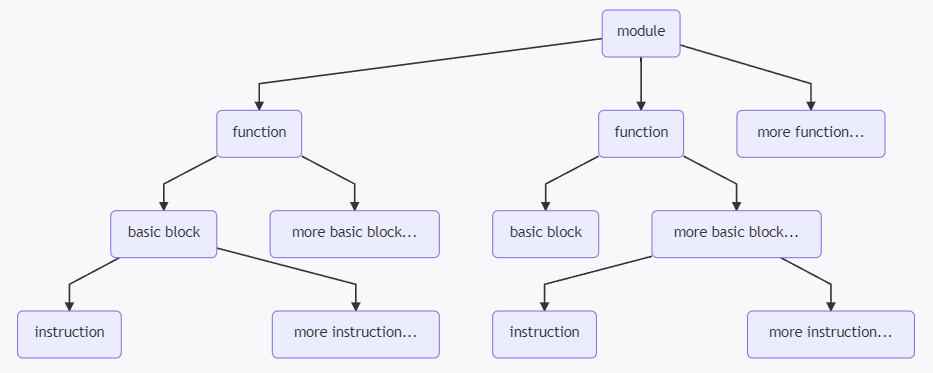
\includegraphics[width=\linewidth]{./Images/BBfunc.png}
    \caption{基本块传参问题\label{fig:BBfunc}}
\end{figure}

\subsubsection{循环部分遇到的问题}

\paragraph{循环的实现}

对于循环语句,我们将其分成3个基本块,count块,body块和end块,在count块进行循环是否结束的判断,在body块是循环体,end块是循环结束后跳转到的块,表示循环语句之后的语句;

当访问到循环语句的分支时,先进入count块(对于repeat语句是body块),判断循环是否结束,进入body块或者end块;body块执行完毕后返回count块;

一个简单的实现如下:

\begin{code}
    \begin{minted}{C++}
auto while_count = llvm::BasicBlock::Create(*llvm_context, "while_count", function, 0); // 创建基本块

builder.CreateBr(while_count); // 无条件跳转
builder.SetInsertPoint(while_count); // 这个语句表示,此后的语句都将作为while_count块的语句,除非跳转到另一块
auto cmp = builder.CreateICmpSLE(tmp_i, final); // 比较
builder.CreateCondBr(cmp, while_body, while_end); // 有条件跳转
\end{minted}
\end{code}

\mintinline{Pascal}{repeat}循环的判断过程中应该使用相反的跳转函数,即当满足条件时跳出循环,当不满足条件时继续执行循环体内容。

在开始构建\mintinline{Pascal}{while}循环的代码块之前便获取了判断条件对应的值,导致在循环过程中若出现对于循环条件的改变,循环体并不能及时获取到对应的循环条件,导致循环体不能正确弹出,在后来的改进过程中,将循环体的条件获取部分延后至循环体的body部分,从而使得每次更新循环条件后都可以正确更新循环条件,使其正确结束循环。

在循环相关函数的初始参数中均存在\mintinline{C++}{llvm::Function *function}部分,这部分代码在传入过程中因为疏忽导致了前面传入的部分为缺省值(指针为空),导致循环体始终出现段错误,在传入正确的指针后循环部分恢复正常。

\subsubsection{段错误的处理}

在代码实现以及测试阶段,我们常常会遇到段错误(Segmentation Fault),段错误究根到底就是访问了非法内存,在实际操作过程中,我们建议使用如下方式去排查段错误:

\begin{enumerate}
    \item 检查数组是否越界
    \item 检查是否使用了空指针来调用函数
    \item 特别的,如果在测试时出现在\mintinline{C++}{createLoad}和\mintinline{C++}{createStore}操作时报告段错误,那么多半是因为你在某个地方用空指针调用了LLVM的函数;对于这样的情况,首先把语句附近所有的指针的值都打印出来,观察是否有空指针;然后对于使用到的作为参数传递的指针,你是否忘记在上一层进行传参,或者在定义函数时,将该参数缺省为0;
\end{enumerate}

这些是我们遇到的,导致段错误的原因,解决这些问题花费了我们不少时间,如果在写代码的时候更规范一些,我们就可以减少类似的问题。

\section{实验总结}

\paragraph{李康童} 本次实验,通过对ANTLR,LLVM工具的学习,我们完成了一个PASCAL-S编译器的编写,在这个过程中,学习掌握了编译相关工具的使用(包括ANTLR,LLVM),并且对于代码开发过程中的代码规范和代码管理的工具更加熟悉(如Docker,GitHub)。

另外,我详细了解了一个编译器的运行过程,包括词法分析,语法分析,中间代码生成等,对编译原理课程的知识学以致用并且有了更加深刻的理解。

在编写代码的过程中,尤其是使用LLVM相关函数API时,遇到的很多问题都找不到比较详细的文档资料来解答,并且查找到的资料大多也是英文的,因此这次实验也提升了我们对于英文文献的阅读理解能力。

\paragraph{班建龙} 这次课设让我学习到了Docker,ANTLR和LLVM的相关知识,同时也加强了我对Git的运用与掌握,了解了团队开发项目的流程和操作。

特别是在编写LLVM相关代码进行语义分析的过程中,我充分的体会到上学期编译原理课程中所学的理论知识,尤其是写到基本块内容以及它们之间的顺序执行,跳转执行时,感受尤深,这也使得我对控制流图的相关内容有了更深刻的理解,以及为后面对基本块进行优化时提供了理论支持。

而后期编写代码时阅读LLVM官方文档也增强了我的英文文档阅读能力,同时也使我对LLVM的基本组成部分:Module、Function、BasicBlock、Instruction以及它们间的关系有了更全面的理解,走完整个课程设计的过程我觉得我对LLVM应该是有了初步的掌握,同时也对上学期所学的编译原理的理论知识进行了实践运用。

\paragraph{毛子恒} 本次实验我们实现了一个简单的Pascal-S语言编译器,将上学期所学习的编译原理知识应用到实际项目中,使我对相关的原理知识有了更加深入的理解和体会。

在编程过程中,我们利用了成熟的开发工具,包括Git、Docker、CMake等,使开发效率和组内写作效率得到大幅提升,我在此期间收获良多。这些工具的熟练使用一定会对我将来的软件开发提供非常大的帮助。

最后,我们在ANTLR和LLVM代码编写过程中,参考许多国外论坛和英文文档,使得自己的英文文档阅读能力得到极大增强。

\paragraph{谢澳伦} 通过这一次课程设计,我不但复习并巩固了上个学期理论课的内容并将一些疑问和想法在行动中践行并解决,对一个前后端分离型的编译器结构及其运作流程有了更加深刻的认识和理解。

在代码过程中,我初步学习使用LLVM构建编译器、应用Docker和Git的相关知识、调整并完善了日常的C++开发环境、使用非集成开发环境进行代码调试,

由于编写代码的过程中,遇到的问题几乎全部只有LLVM官网的自动生成文档可以参考,不仅我提高了自己的英文文档阅读水平和大型结构图的阅读理解能力,还更加积极的参与团队合作中相关问题的讨论。

\paragraph{李俊辉} 通过本次编译原理课程设计,对于一套完整的编译器制作流程有了进一步的认识,从最开始的ANTLR生成的Pascal-S语法树,到后面通过Visitor模式的语法树遍历,然后通过LLVM工具将语法树转变为中间代码然后生成可执行文件,整个过程较好复现了编译原理这门课程对于一种语言实现的前端与后端,对于整体的实现流程有了更加深刻的见解。

对于ANTLR部分的语法树学会了通过ANTLR语法的g4文件描述Pascal-S语法,采用的类BNF范式较好描述了一种语言的语法规则,按照形式语言与自动机的理解方式,将这门语言较好的描述出来,不仅是对于Pascal-S语法的描述,后续对于其他已知语法的语言也可以采用相同的逻辑方式。

对于Visitor部分,LLVM工具的使用让编译器实现了从前端语法树到后端中间代码的转变,从Scope变量表的存储到每一部分语法树的遍历,既是对Pascal-S语法的进一步深刻认知,也是对于自动机以及正则式的进一步理解,更好实现了不同学科之间的联系。

在整个实现过程中出现的错误大部分为指针错误(包括空指针,指向错误等问题),对于小型项目的代码安排有了更加深切的体会,同时小组合作的模式也让我对于团队合作实现项目有了更加好的锻炼,对于项目整体规划、功能模块分工合作有了更加深刻的认知。

\paragraph{乔永琦} 通过本次编译原理课程设计,我加深了对编程语言底层实现的理解,对LLVM、ANTLR、Docker的掌握也更加完整。

本次课程设计的关键点在于Pascal-S语言的词法分析器、语法分析器的设计,分析过程中涉及的多种需要自己实现的功能,同时也对我们编写代码、调试代码的能力有更高的要求。与上学期编译的实验相比,对一种语言设计一个完整的编译器有更高的难度,如果对词法、语法、语义等知识点一知半解,则很难理解程序原理和调试。

在本次课程设计过程中,我们灵活运用多种程序调试方式:观察LLVM IR代码、通过添加输出信息、读取LLVM地址信息等⋯⋯当然,其中最基础也是重要的还是查看LLVM IR的代码,检查函数、基本块、变量等是否出现异常。

调试程序、发现错误、找出根源的过程锻炼了我们遇到问题坚持不懈的品质,增强了我们面对程序时的耐心和毅力。在此过程中我们碰撞出了思维的火花,相互帮助学习,每一位成员都受益良多。

\appendix

\section{Pascal-S语法}

\label{PascalS}

\begin{code}
    \begin{minted}{text}
program
   => programHeading block DOT
   
programHeading
   => PROGRAM identifier (LPAREN identifierList RPAREN)? SEMI
   
identifier
   => IDENT
   
block
   => (constantDefinitionPart | typeDefinitionPart | variableDeclarationPart | procedureAndFunctionDeclarationPart)* compoundStatement
   
constantDefinitionPart
   => CONST (constantDefinition SEMI)+
   
constantDefinition
   => identifier EQUAL constant
   
constant
   => unsignedNumber         
   | sign unsignedNumber    
   | identifier             
   | sign identifier        
   | string                 
   
unsignedNumber
   => unsignedInteger    
   | unsignedReal       
   
unsignedInteger
   => NUM_INT
   
unsignedReal
   => NUM_REAL
   
sign
   => PLUS   
   | MINUS  
   
bool_
   => TRUE   
   | FALSE  
   
string
   => STRING_LITERAL
   
typeDefinitionPart
   => TYPE (typeDefinition SEMI)+
   
typeDefinition
   => identifier EQUAL type_
   
type_
   => simpleType     
   | structuredType 
   
simpleType
   => (CHAR | BOOLEAN | INTEGER | REAL)
   
structuredType
   => arrayType  
   | recordType 
   
arrayType
   => ARRAY LBRACK periods RBRACK OF type_   
   | ARRAY LBRACK2 periods RBRACK2 OF type_ 
   
periods
   => period (COMMA period)*
   
period
   => constant DOTDOT constant
   
recordType
   => RECORD recordField? END
   
recordField
   => variableDeclaration (SEMI variableDeclaration)* SEMI
   
variableDeclarationPart
   => VAR variableDeclaration (SEMI variableDeclaration)* SEMI
   
variableDeclaration
   => identifierList COLON type_
   
procedureAndFunctionDeclarationPart
   => procedureOrFunctionDeclaration SEMI
   
procedureOrFunctionDeclaration
   => procedureDeclaration   
   | functionDeclaration    
   
procedureDeclaration
   => PROCEDURE identifier (formalParameterList)? SEMI block
   
formalParameterList
   => LPAREN formalParameterSection (SEMI formalParameterSection)* RPAREN
   
formalParameterSection
   => parameterGroup     
   | VAR parameterGroup 
   
parameterGroup
   => identifierList COLON simpleType
   
identifierList
   => identifier (COMMA identifier)*
   
constList
   => constant (COMMA constant)*
   
functionDeclaration
   => FUNCTION identifier (formalParameterList)? COLON simpleType SEMI block
   
statement
   => simpleStatement        
   | structuredStatement    
   
simpleStatement
   => assignmentStatement    
   | procedureStatement     
   | emptyStatement_        
   
assignmentStatement
   => variable ASSIGN expression
   
variable
   => identifier (LBRACK expression (COMMA expression)* RBRACK | LBRACK2 expression (COMMA expression)* RBRACK2 | DOT identifier)*
   
expression
   => simpleExpression (relationaloperator simpleExpression)?
   
relationaloperator
   => EQUAL      
   | NOT_EQUAL  
   | LT         
   | LE         
   | GE         
   | GT         
   
simpleExpression
   => term (additiveoperator term)?
   
additiveoperator
   => PLUS   
   | MINUS  
   | OR     
   
term
   => signedFactor (multiplicativeoperator signedFactor)?
   
multiplicativeoperator
   => STAR   
   | SLASH  
   | DIV    
   | MOD    
   | AND    
   
signedFactor
   => (PLUS | MINUS)? factor
   
factor
   => variable                   
   | LPAREN expression RPAREN   
   | functionDesignator         
   | unsignedConstant           
   | NOT factor                 
   | bool_                      
   
unsignedConstant
   => unsignedNumber 
   | string         
   
functionDesignator
   => identifier LPAREN parameterList RPAREN
   
parameterList
   => actualParameter (COMMA actualParameter)*
   
procedureStatement
   => identifier (LPAREN parameterList RPAREN)?
   
actualParameter
   => expression parameterwidth*
   
parameterwidth
   => '=>' expression
   
emptyStatement_
   =>
   
empty_
   =>
   /* empty */
   
structuredStatement
   => compoundStatement      
   | conditionalStatement   
   | repetetiveStatement    
   
compoundStatement
   => BEGIN statements END
   
statements
   => statement (SEMI statement)*
   
conditionalStatement
   => ifStatement    
   | caseStatement  
   
ifStatement
   => IF expression THEN statement (=> ELSE statement)?
   
caseStatement
   => CASE expression OF caseListElement (SEMI caseListElement)* (SEMI ELSE statements)? END
   
caseListElement
   => constList COLON statement
   
repetetiveStatement
   => whileStatement     
   | repeatStatement    
   | forStatement       
   
whileStatement
   => WHILE expression DO statement
   
repeatStatement
   => REPEAT statements UNTIL expression
   
forStatement
   => FOR identifier ASSIGN forList DO statement
   
forList
   => initialValue (TO | DOWNTO) finalValue
   
initialValue
   => expression
   
finalValue
   => expression
   
recordVariableList
   => variable (COMMA variable)*

PLUS
   => '+'
   
MINUS
   => '-'
   
STAR
   => '*'
   
SLASH
   => '/'
   
ASSIGN
   => '=>='
   
COMMA
   => ','
   
SEMI
   => ';'
   
COLON
   => '=>'
   
EQUAL
   => '='
   
NOT_EQUAL
   => '<>'
   
LT
   => '<'
   
LE
   => '<='
   
GE
   => '>='
   
GT
   => '>'
   
LPAREN
   => '('
   
RPAREN
   => ')'
   
LBRACK
   => '['
   
LBRACK2
   => '(.'
   
RBRACK
   => ']'
   
RBRACK2
   => '.)'
   
DOT
   => '.'
   
DOTDOT
   => '..'
   
LCURLY
   => '{'
   
RCURLY
   => '}'

IDENT
   => ('a' .. 'z' | 'A' .. 'Z') ('a' .. 'z' | 'A' .. 'Z' | '0' .. '9' | '_')*

STRING_LITERAL
   => '\'' ('\'\'' | ~ ('\''))* '\''

NUM_INT
   => ('0' .. '9') +

NUM_REAL
   => ('0' .. '9') + (('.' ('0' .. '9') + (EXPONENT)?)? | EXPONENT)

EXPONENT
   => ('e') ('+' | '-')? ('0' .. '9') +
\end{minted}
\end{code}

\end{document}